\section{Intelligent Systems}
\subsection{Computing machinery and intelligence}

\par
The course starts by reading Turing's article \textit{``Computing machinery and intelligence''}, published on the Mind journal in October 1950 \cite{10.1093/mind/LIX.236.433}. In it, Turing complains about the intrinsic ambiguity of the question ``can machines think?'', which relies on the definition of both ``machine'' and ``think''. To reformulate this problem by means of less ambiguous words, he introduces \textbf{the imitation game}, in which an interrogator (C) tries to guess by asking questions and receiving answers, which of the other two participants (that are in a different room and that he only knows by means of the labels X and Y) is a man (A) and which is a woman (B). A's goal is to cause C to make the wrong identification, while B's goal is to help the interrogator. To limit the number of indirect clues that the interrogator may have, the answers should be typewritten or repeated by an intermediary.

\par
Turing then suggests replacing the previous question with a new one: \textit{``what will happen when a machine\footnote{Later he restricts the definition of machine to digital computers} takes the part of A in this game? Will the interrogator decide wrongly as often when the game is played like this as he does when the game is played between a man and a woman?''}. In a later part of his article, he clarifies that the goal of the game is not to find out \textit{``whether all digital computers would do well in the game nor whether the computers at present available would do well, but whether there are imaginable computers which would do well''}.

\par
In the last chapter, Turing proposes a few solutions on how to tackle the problem of learning machines (which he argues to be a programming problem); he starts by analyzing the human brain, which he says has three components:
\begin{itemize}
    \item The initial state of the mind (say at birth).
    \item The education to which it has been subjected.
    \item Other experience, not to be described as education, to which it has been subjected.
\end{itemize}
Instead of producing a program to simulate an adult mind, he suggests producing one that simulates a child's brain and subject it to an appropriate ``education'' to obtain an adult brain. He is very aware that \textit{``we cannot expect to find a good child machine at the first attempt. One must experiment with teaching one such machine and see how well it learns. One can then try another and see if it is better or worse. There is an obvious connection between this process and evolution [...]''}. The teaching process will have to involve punishments and rewards: \textit{``the machine has to be so constructed that events which shortly preceded the occurrence of a punishment signal are unlikely to be repeated, whereas a reward signal increased the probability of repetition of the vents which led up to it''}. Finally, he also foresees one of the problems that is still unsolved in the machine learning field: \textit{``an important feature of a learning machine is that its teacher will often be very largely ignorant of quite what is going on inside, although he may still be able to some extent to predict his pupil's behavior''}.

\subsection{Intelligent machines}
After seeing a few examples of autonomous systems, like self-driving cars and agents that play videogames, it is clear that our goal is to be able to build machines that can learn from experience, trying things out on their own, without any human intervention. We first start by giving some definitions.

\subsubsection{Intelligent agents}
We define an \textbf{intelligent agent} as an entity that perceives its environment and takes actions that maximize the probability of achieving its goals. It is important to note that the agent does not know what set of actions will allow it to reach the goal, it just ``moves'' towards actions that maximize the probability of it happening. Agents may also be physically situated (we call them \textbf{robots}) or not (we refer to them as \textbf{software agents} or \textbf{bots}).

\subsubsection{Adaptive agents}
We define an \textbf{adaptive agent} as an entity that can respond to changes in its environment. This is possible thanks to a lack of determinism: the agent will adapt and react to the environment (which may also include other agents) and take different actions.

Learning can take place in various ways: at the end of a generation, with \textbf{natural selection} and the survival of the fittest, or during a generation, with a method that is more similar to \textbf{reinforcement learning}.

\subsubsection{Autonomous agents}
We define an \textbf{autonomous agent} as an entity that only relies on its perception and acts in the world independently from its designer. A key characteristic of this type of agent is that they should be able to compensate for partial knowledge: in the beginning they may only know how to perceive the environment and how to take a certain set of actions; from a practical point of view, it makes sense to provide the agent with some knowledge of the world and the ability to learn. After sufficient experience of its environment, an intelligent agent can become effectively independent of its prior knowledge.

\subsubsection{Designing agents}
When designing agents, we need to take into consideration the following dimensions:
\begin{itemize}
    \item Performance: how ``good'' is the agent.
    \item Environment: what is ``around'' the agent.
    \item Actuators: how the agent can take actions in the environment.
    \item Sensors: how the agent perceives the environment.
\end{itemize}

A schema of how these dimensions are linked can be found in figure \ref{fig:ch1-agentenvironmentschema}, along with a few examples of agents in figure \ref{fig:ch1-agentexamples}.

\begin{figure}[hbt]
    \centering
    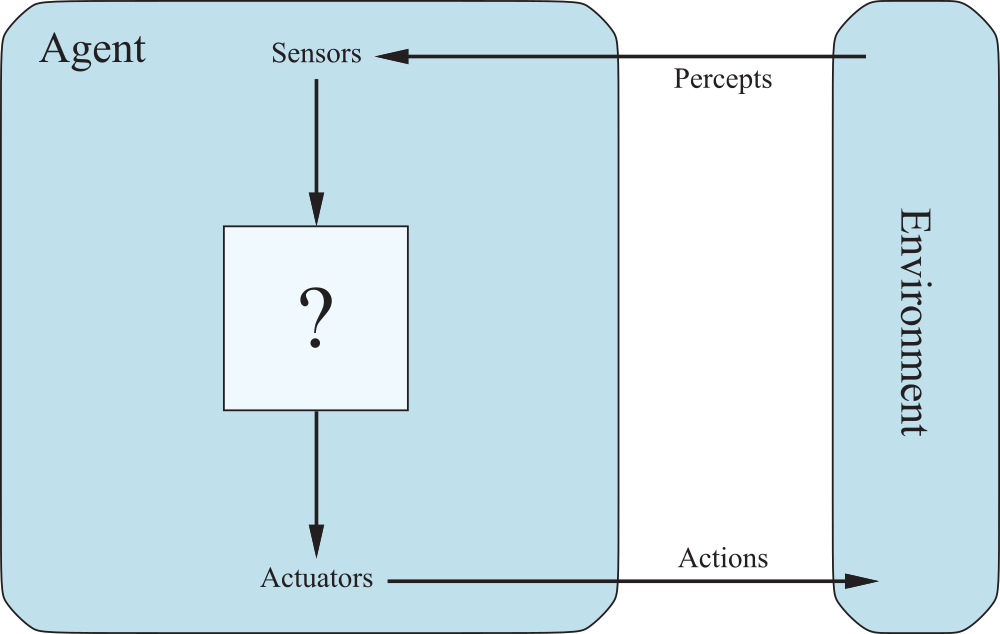
\includegraphics[scale=0.35]{Images/Chapter 1/agent-environment-schema.png}
    \caption{Schema of the interaction between an agent and the environment.}
    \label{fig:ch1-agentenvironmentschema}
\end{figure}
\begin{figure}[hbtp]
    \centering
    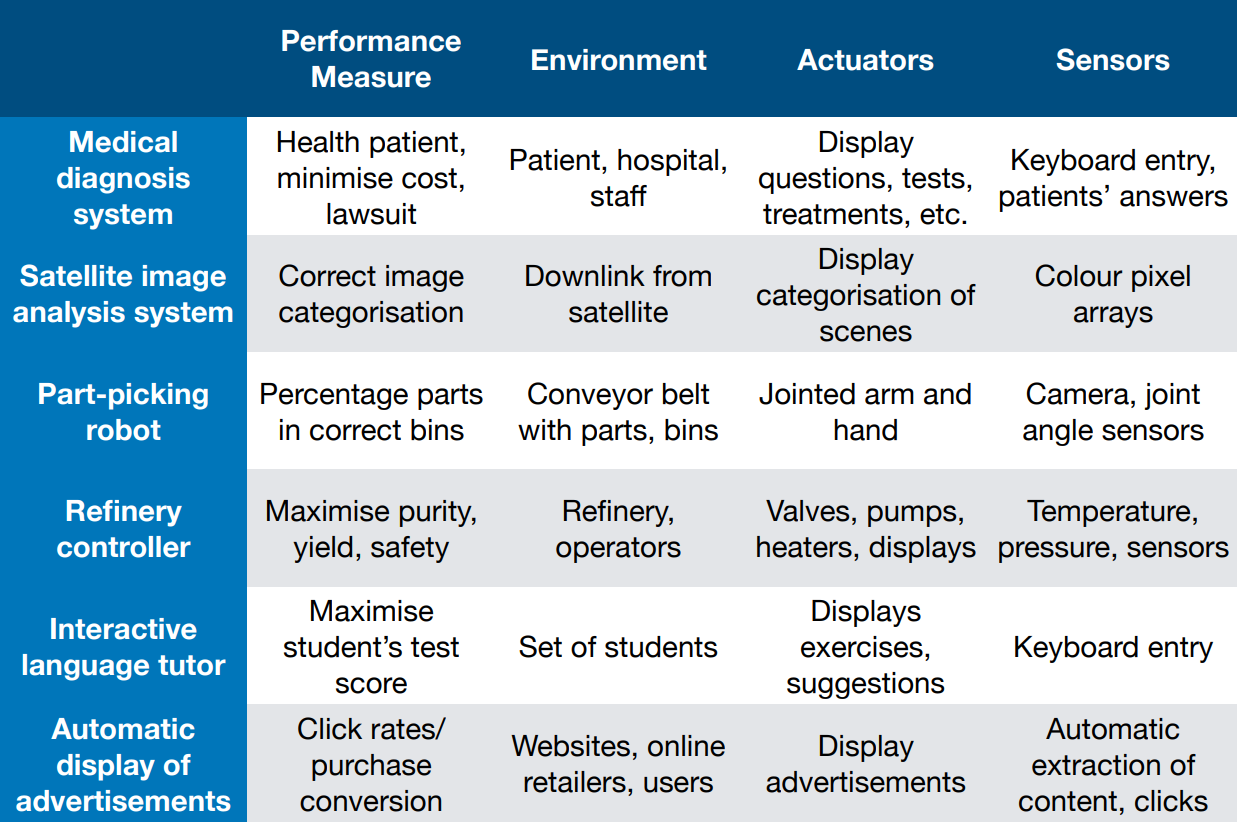
\includegraphics[width=\textwidth]{Images/Chapter 1/agents-type.png}
    \caption{Examples of agents and their characteristics.}
    \label{fig:ch1-agentexamples}
\end{figure}

\subsection{Characteristics of the environments}
The environment in which our agent is in may be of different types:
\begin{itemize}
    \item \textbf{Fully observable vs partially observable}: we may or may not be able to see the entire environment (e.g., there may be occlusions limiting our sight).
    \item \textbf{Deterministic vs stochastic}: the environment may be predictable (e.g., governed by the laws of Newtonian physics) or not (e.g., the environment may be changed by another agent).
    \item \textbf{Episodic vs sequential}: the environment may be divided in “episodes” that have a beginning and an end (e.g., the levels of a game) or open-ended (e.g., a self-driving car that keeps driving).
    \item \textbf{Static vs dynamic}: the environment may or may not change over time (an action that we take now could have a different result compared to when we took it in the past, e.g., certain agents with whom we collaborated in the past, may not do so anymore; driving in dry conditions is different compared to driving in the rain or in the snow).
    \item \textbf{Discrete vs continuous}: the environment may be discrete or continuous (e.g., the wind speed is a continuous attribute of the environment).
    \item \textbf{Single agent or multi-agent}: there may be multiple agents in the environment, and we may want them to collaborate.
\end{itemize}

\subsection{A categorization of intelligent agents}
There are essentially four basic kinds of agent programs:
\begin{itemize}
    \item \textbf{Simple reflex agents}.
    \item \textbf{Model-based reflex agents}.
    \item \textbf{Goal-based agents}.
    \item \textbf{Utility-based agents}.
\end{itemize}
The behavior of these agents can be hard-wired or it can be acquired, improved and optimized through learning.

\subsubsection{Simple reflex agents}
Simple reflex agents select actions on the basis of the current perceptions, ignoring the perception history. They are the most basic form of agents and are based on condition-action rules (also called simulation-action rules, productions, or if-then rules). (See figure \ref{fig:ch1-simplereflexagent})

\begin{figure}[hbt]
    \centering
    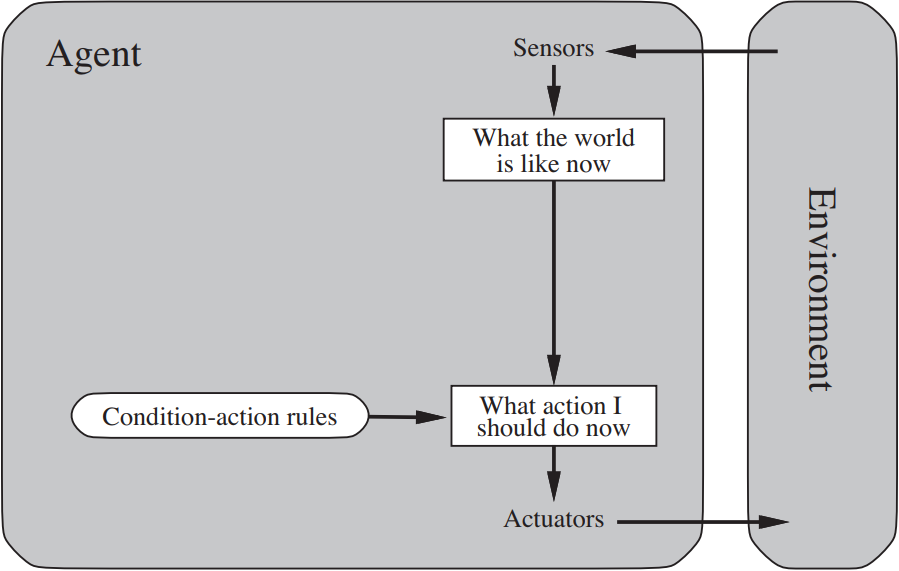
\includegraphics[scale=0.35]{Images/Chapter 1/simple-reflex-agents.png}
    \caption{Schema of a simple reflex agent.}
    \label{fig:ch1-simplereflexagent}
\end{figure}

\subsubsection{Model-based reflex agents}
Model-based agents keep an internal state and depend on two types of knowledge:
\begin{itemize}
    \item How the world evolves independently from the agent (e.g., the trajectory that a bullet/a stone follows when shot/thrown).
    \item How the actions of the agent affect the world (e.g., if I turn the wheel to the right, the car moves to the right).
\end{itemize}
The internal state is essentially used to keep track of what it is not possible to see/perceive right now. It depends on the perception history and, for this reason, it reflects at least some of the unobserved aspects of the current state. (See figure \ref{fig:ch1-modelbasedreflexagent})

\begin{figure}[hbt]
    \centering
    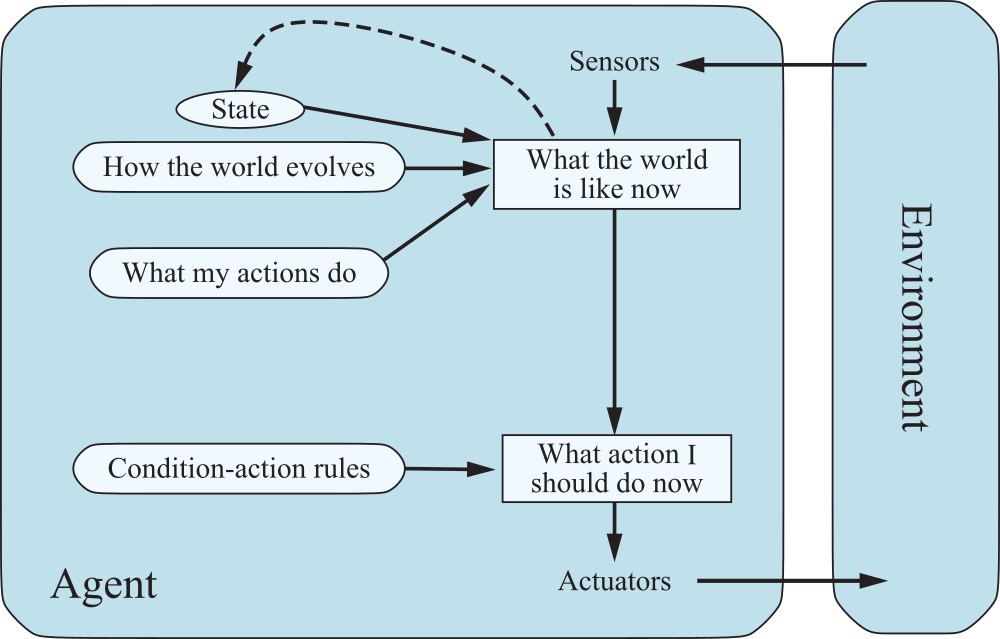
\includegraphics[scale=0.35]{Images/Chapter 1/model-based-reflex-agent.png}
    \caption{Schema of a model-based reflex agent.}
    \label{fig:ch1-modelbasedreflexagent}
\end{figure}

\subsubsection{(Model-based) Goal-based agents}
Goal-based agents act in order to achieve their goals. If we can achieve the goal by carrying out a single action, goal-based action selection is straightforward; in the other cases, the agent needs to consider a long sequence of actions by means of search and planning. (See figure \ref{fig:ch1-goalbasedagent})

\begin{figure}[hbt]
    \centering
    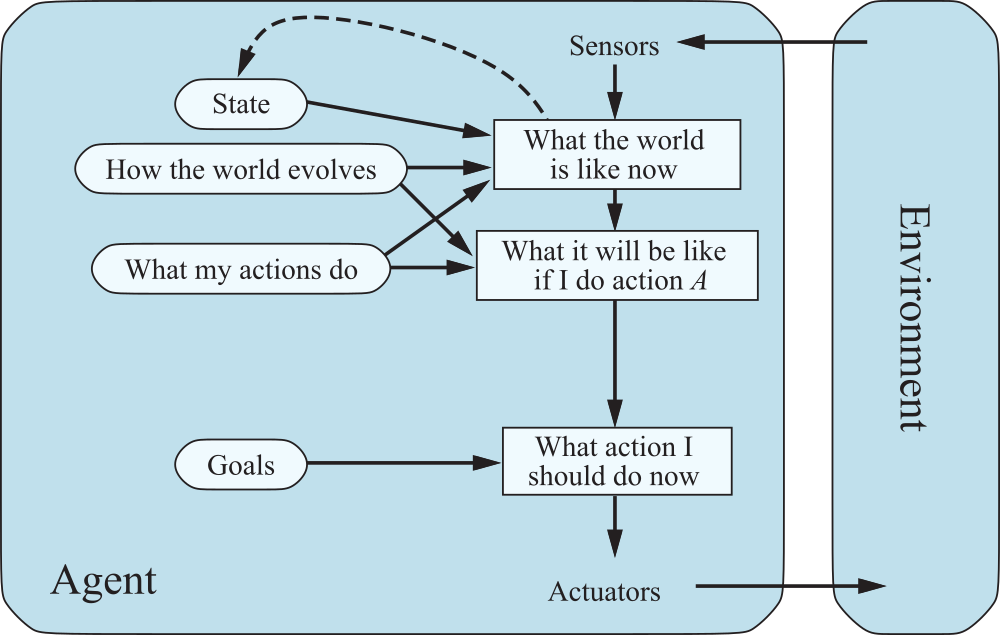
\includegraphics[scale=0.35]{Images/Chapter 1/goal-based-agent.png}
    \caption{Schema of a goal-based agent.}
    \label{fig:ch1-goalbasedagent}
\end{figure}

\subsubsection{(Model-based) Utility-based agents}
Goals are not sufficient to generate “high-quality behavior” in most environments, since there are usually states that are preferrable to others. In order to code this “preference”, we use utility functions that map a state (or a sequence of states) to a real number (e.g., we want to get to a destination by following the shortest or quickest path). (See figure \ref{fig:ch1-utilitybasedagent})

Note that how to model these preferences is one of the current unsolved and “hot” topics in the artificial intelligence field.

\begin{figure}[hbt]
    \centering
    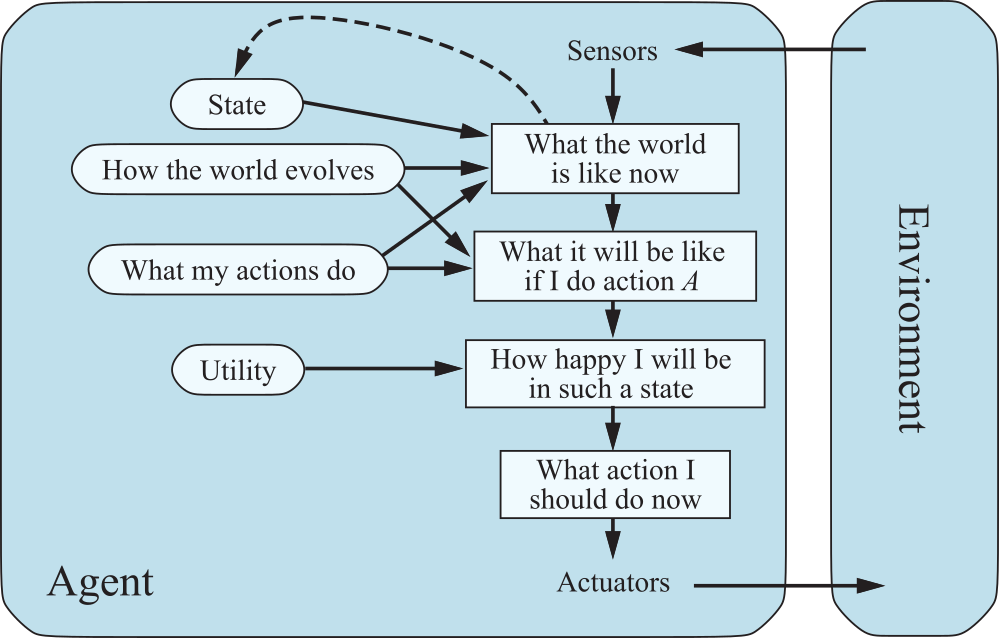
\includegraphics[scale=0.35]{Images/Chapter 1/utility-based-agent.png}
    \caption{Schema of a utility-based agent.}
    \label{fig:ch1-utilitybasedagent}
\end{figure}

To conclude this first introduction, we now have a look at learning.

\subsection{Learning}
As we have said before, the behavior of the agents can be pre-programmed (hard-wired, fixed) or it can be learned by means of a learning component. This component can be based on a model of the world and the gain towards a certain goal (possibly expressed in terms of the change of the value of utility functions) can be expressed through rewards. This behavior is at the basis of the type of learning that we will explore in detail in this course, called \textbf{reinforcement learning}. Following Herbert Simon’s definition of autonomous and adaptive systems, we will consider \textit{``machines that think, that learn and that create''}.